\section{SaltProc}

SaltProc is the online reprocessing simulation
driver for SERPENT2 \cite{leppanen_serpent_2015},
for simulating liquid-fueld \gls{MSR} operation [??? new zenodo].
SaltProc uses a semi-continuous approach to simulate
continuous \gls{MSR} material feed and removal \cite{rykhlevskii_online_2017}.
It is coded in Python (compatible both in 2.7 and 3.6), and
outputs an HDF5 \cite{the_hdf_group_hierarchical_1997} database
with feed, removal and in-core isotopic history.

SaltProc's structure and capabilities are similar to that of the
ChemTriton tool for SCALE, developed in ORNL \cite{betzler_molten_2017}.
The computationally heavy work - Monte Carlo neutron transport and
burnup calculations - are done in SERPENT, while SaltProc parses through
the output material compositions, processes the fuel (removal and feed),
and creates a new SERPENT input. The user can specify removal and feed
rates and removal efficiencies for each material stream. At each
timestep, the material compositions after the
depletion calculation and after fuel processing are recorded in the
database, as well as the feed and removal stream. 

The logic flow of SaltProc is illustrated in figure \ref{fig:SaltProc}.
Initially, SaltProc reads a user-defined SERPENT 2 input file that
contains input cards with parameters such as  geometry, non-fuel components' composition,
neutron population, criticality cycles, depletion time, total power, and boundary conditions.
SERPENT 2 then performs neutron transport and depletion calculations, and 
returns the number density of the depleted fuel. SaltProc then reads the
depleted composition, writes the composition in the database, processes
the depleted material according to a user-defined scheme, and then
outputs a new fuel composition input card for SERPENT 2. This again
is then read by SERPENT 2 and the cycle continues until the user-defined
timestep is reached.

\begin{figure}[htbp!]
	\begin{center}
		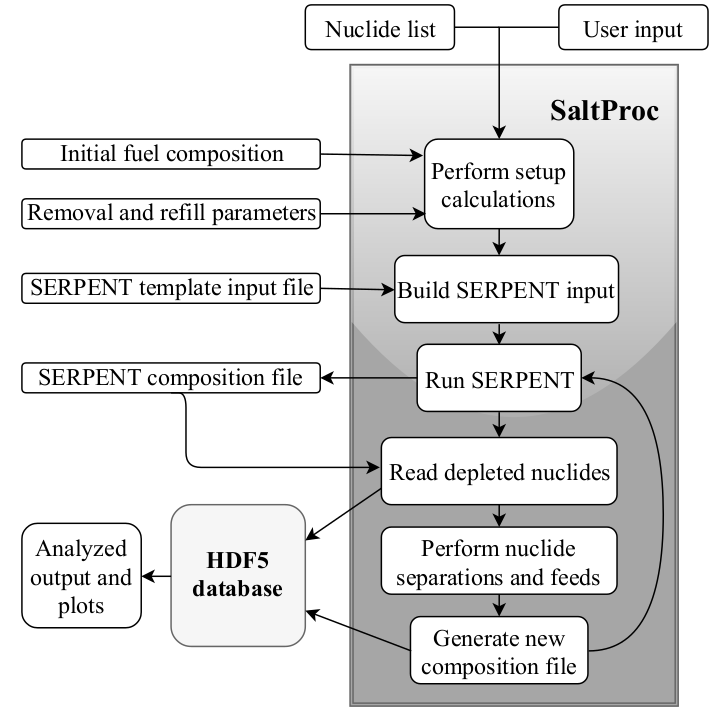
\includegraphics[scale=0.3]{./images/saltproc.png}
	\end{center}
	\caption{Flow chart for the SaltProc tool
		\cite{rykhlevskii_online_2017}.}
	\label{fig:SaltProc}
\end{figure}


One of the benefits of having a semi-continuous external driver for
SERPENT 2 is that the user can set up SaltProc so that the density
of a certain isotope in the fuel remains constant. In other words,
the feed rate can vary over time to meet a certain `quality' of the fuel.
Also, using a Monte Carlo code such as SEPRENT allows users to vary
in geometric fidelity, from a single cell model to a full core model.

\subsection{Usage in this work}
SaltProc's output, the HDF5 database can be imported through a Cyclus
module, where the module can mimic the \gls{MSR} feed and removal
behavior throughout its lifetime. The composition in the core can
be ignored, since the data of interest for a system-level \gls{NFC} simulation
is the material flow in and out of the reactor. This method can
then effectively model \glspl{MSR} in a large system-scale \gls{NFC}
simulation without a large computational burden for the \gls{NFC} simulation.